% ============================================================
% Marital Insurance and Job Search: Evidence from Property
% Regime Reform
% Sofia Valdivia & Heleen Ren | Feb. 2026
% ============================================================
\documentclass[aspectratio=169, 11pt]{beamer}

% ---------- Theme & Colors ----------------------------------
\usetheme{Madrid}
\usecolortheme{seahorse}
%\setbeamercolor{palette primary}{bg=darkblue,fg=white}
%\setbeamercolor{palette secondary}{bg=darkblue!80,fg=white}
%\setbeamercolor{palette tertiary}{bg=darkblue!60,fg=white}
%\setbeamercolor{palette quaternary}{bg=darkblue,fg=white}
%\setbeamercolor{structure}{fg=darkblue}
\setbeamercolor{block title}{bg=darkblue,fg=white}
\definecolor{darkblue}{RGB}{0,51,102}
\definecolor{highlight}{RGB}{220,80,60}
\newcommand{\highlight}[1]{\textcolor{blue!80!black}{\textbf{#1}}}

\setbeamertemplate{navigation symbols}{}
\setbeamertemplate{footline}[frame number]
\setbeamertemplate{title page}[default][colsep=-4bp,rounded=true]

\usepackage{appendixnumberbeamer}
\usepackage{booktabs}
\usepackage{amsmath,amssymb}
\usepackage{xcolor}
\usepackage{pgfplots}
\pgfplotsset{compat=1.18}
\usepackage{tikz}
\usetikzlibrary{arrows.meta, calc, positioning, shapes.geometric, decorations.pathreplacing}
\usepackage{hyperref}
\usepackage{comment}
\usepackage{natbib}
%\usepackage[style=ext-authoryear, backend=biber, giveninits=true, uniquelist = false, uniquename=init, isbn=false, maxcitenames=1, dashed=false, maxbibnames=999, doi=false, url=false]{biblatex}
%\addbibresource{bib.bib}

\definecolor{dutch}{RGB}{0,70,127}       % deep Dutch blue
\definecolor{dutchlight}{RGB}{210,230,248}
\definecolor{orange}{RGB}{214,90,0}
\definecolor{gray80}{RGB}{80,80,80}


\newcommand{\R}[1]{\textcolor{orange}{\textbf{#1}}}
\newcommand{\B}[1]{\textcolor{dutch}{\textbf{#1}}}
\newcommand{\wR}{w^R}
\newcommand{\aJ}{a^J}
\newcommand{\aD}{a^D}

% ---------- Title -------------------------------------------
\title{\textbf{Marital Insurance and Job Search}}
\subtitle{Evidence from Property Regime Reform}
\author{Sofia Valdivia \and Heleen Ren}
\date{Structural Methods in Labor — February 2026}
\institute{}

% ============================================================
\begin{document}
% ============================================================

\maketitle

% ------------------------------------------------------------
\section{Motivation}
% ------------------------------------------------------------

\begin{frame}{The Core Question}
\textbf{A well-known fact:} married individuals search for jobs differently than singles.
\vspace{0.2em}
\begin{itemize}
  \item Higher reservation wages \citep{GULER2012352}
  \item Faster job-ladder climbing \citep{pilossoph_wee}
  \item Greater willingness to take labor market risk \citep{FERNANDEZBLANCO2022105477}
\end{itemize}
\vspace{1.6em}
\textbf{Why?} 
Canonical explanation is that spousal income provides \highlight{insurance}. \\
$\Rightarrow$ However, existing literature treats marital insurance as fixed
\vspace{2.0em}

\textbf{This paper asks}: Does the strength of marital insurance — governed by the matrimonial property regime — causally shape household job search behavior? \\
% think if want to phrase it like this or as asset ownership
$\Rightarrow$ Exploit the 2018 Dutch reform changing the default from \emph{universal} to \emph{limited} community property.

\end{frame}

% ------------------------------------------------------------
\section{Why a Structural Model?}
% ------------------------------------------------------------

\begin{frame}{Why We Need a Structural Model}
\textbf{Reason 1: Marital insurance is unobservable.}\\[0.3em]
Property regimes change divorce payoffs, but the effect on job search comes from:
\begin{columns}[T]
\begin{column}{0.48\textwidth}
\begin{itemize}
  \item Forward-looking expectations about income risk
  \item Anticipated divorce probability
  \item Asset accumulation and savings decisions
\end{itemize}
\end{column}
\begin{column}{0.50\textwidth}
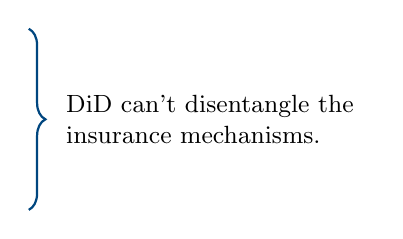
\begin{tikzpicture}
  \draw[decorate, decoration={brace, amplitude=6pt}, thick, dutch]
    (0, 2.35) -- (0, 0.05);
  \node[right=10pt, text width=3.8cm, font=\small] at (0, 1.2)
    {DiD can't disentangle the insurance mechanisms.};
\end{tikzpicture}
\end{column}
\end{columns}
\vspace{1.5em}
\textbf{Reason 2: Job search is dynamic.}\\[0.3em]
Reservation wages, search intensity, and unemployment duration jointly depend on:
\begin{itemize}
  \item Value of remaining unemployed
  \vspace{0.1cm}
  \item Wage offer distribution
  \vspace{0.1cm}
  \item Continuation value of marriage
  \vspace{0.1cm}
  \item Asset path
\end{itemize}
%\vspace{0.3em}
%\B{Structural model allows:}
%\begin{enumerate}
%  \item Discipline all channels simultaneously
%  \item Counterfactual policy analysis
%  \item Welfare implications
%\end{enumerate}
\end{frame}

% ------------------------------------------------------------
%\begin{frame}{Why This Matters}
%\textbf{Conceptual contribution:}
%\begin{itemize}
%  \item Identifies a specific institutional lever for intra-household insurance
%  \item Separates insurance from other marriage-wage effects (specialization, selection)
%\end{itemize}
%\begin{alertblock}{Main mechanism}
%\small
%Weaker property regime $\Rightarrow$ lower effective insurance $\Rightarrow$ forward-looking couples internalize divorce risk $\Rightarrow$ lower reservation wages, less job-ladder risk-taking — even \emph{while still married}.
%\end{alertblock}
%\vspace{0.5em}
%\small
%Anticipation effects are \emph{invisible} to reduced-form methods. They require a structural model.
%\end{frame}

% ------------------------------------------------------------
\section{Institutional Background}
% ------------------------------------------------------------

\begin{frame}{Dutch Matrimonial Property Regimes}
Two regimes:
\vspace{0.3em}

\textbf{Universal Community Property (U):}
\begin{itemize}
  \item All assets (premarital, inherited, gifted) $\to$ jointly owned
  \item Equal division upon divorce %(minus dissolution costs $\tau_U > 0$)
  \item Default in NL \textbf{before 2018}
\end{itemize}
\vspace{0.4em}
\textbf{Limited Community Property (L):}
\begin{itemize}
  \item Only assets acquired during marriage are jointly owned
  \item Pre-marital assets, inheritances, gifts $\rightarrow$ separate
  \item Default in NL \textbf{after January 1, 2018}
\end{itemize}
\vspace{0.8em}

\highlight{Interpretation}: Effective marital insurance  $\downarrow$


%\begin{block}{Divorce payoffs}
%\small
%\vspace{0.3em}
%\textbf{Under $\theta = U$:}
%$$a^D_i = \tfrac{1}{2}(1-\tau_U)(a^J + a_m + a_f)$$
%\vspace{0.3em}
%\textbf{Under $\theta = L$:}
%$$a^D_i = \tfrac{1}{2}a^J + a_i$$
%\vspace{0.2em}
%\small
%Under $L$: wealth shocks (inheritances, premarital appreciation) stay \emph{individual} $\Rightarrow$ less pooling.
%\end{block}
\end{frame}

% ------------------------------------------------------------
\begin{frame}{The 2018 Reform as a Natural Experiment}
\textbf{Why the reform is useful:}
\begin{itemize}
  \item Data show $\approx$80\% of married couples remain on the default; no evidence of sorting. 
\end{itemize}
\vspace{0.8em}
\textbf{Identifying variation:}
\begin{itemize}
  \item Treatment: married post-2018 ($L$) vs.\ pre-2018 ($U$)
  \item Interaction: couples with larger individual wealth shocks (inheritances, premarital assets) exposed to bigger reduction in pooling under $L$
\end{itemize}
\vspace{0.8em}
\textbf{Illustrative example:} Individual in household receives an inheritance \\
\begin{itemize}
  \item[$\rightarrow$]Under $U$: an inheritance is split at divorce.\\
  \item[$\rightarrow$]Under $L$: it stays individual.\\
\end{itemize}
Same inheritance $\Rightarrow$ different insurance loss depending on regime $\Rightarrow$ identify the insurance channel.
\end{frame}

% ------------------------------------------------------------
\section{Related Literature}
% ------------------------------------------------------------

\begin{frame}{Literature: Household Job Search}
\small
\begin{tabular}{p{4.2cm} p{8.2cm}}
\toprule
\textbf{Paper} & \textbf{Key insight / what we build on} \\
\midrule
Guler, Guvenen \& Violante (2012) & Joint-search model with location frictions; spousal income as insurance raises $\wR$; breadwinner cycles \\[0.3em]
Mankart \& Oikonomou (2017) & Spousal labor-supply adjustments insure against unemployment \\[0.3em]
Pilossoph \& Wee (2021) & Income pooling raises $\wR$ \emph{and} accelerates job-ladder climbing; marital wage premium \\[0.3em]
Fernández-Blanco (2022) & Consumption insurance from spousal income increases risk-taking \\[0.3em]
Lise (2012) \& Wang (2019) & On-the-job search with savings; search cost functional form \\
\bottomrule
\end{tabular} \\
\vspace{0.5em}
\normalsize
\textbf{Our departure:} We vary the strength of marital insurance through property regime heterogeneity, rather than comparing singles vs.\ couples.
\end{frame}



% ------------------------------------------------------------
\section{Model}
% ------------------------------------------------------------

\begin{frame}{Model: Overview}
\begin{columns}
\begin{column}{0.48\textwidth}
\textbf{Agents:}
\small
\begin{itemize}
  \item Unitary couple $i \in \{m, f\}$
  \item Continuous time, infinite horizon
  \item Maximize $V_0 = E_0\int_0^\infty e^{\rho t} u(c_t)\,dt$
  \item Budget constraint: $c_t + a_{t+1} = (1+r)a_t + y_t$
  %\item CRRA utility, $u''(c) < 0$
\end{itemize}
\vspace{0.4em}
\normalsize
\textbf{State space:} $(w_m, w_f, a^J, a_m, a_f, l_m, l_f, \theta)$
\small
\begin{itemize}
  \item Wages, joint \& individual assets
  \item Employment status pair $(l_m, l_f) \in \{0,1\}$
  \item Property regime $\theta \in \{U, L\}$
\end{itemize}
\end{column}
\begin{column}{0.45\textwidth}
\small
\textbf{Key primitives:}
\begin{itemize}
  \item Job destruction rate $\delta_i$
  \item Unemployment benefit $b_i$
  \item Wage offer distribution $F_i(w)$ on $[\underline{w}_i, \overline{w}_i]$
  \item Offer arrival (unemployed) $\lambda_i$; on-job $\gamma_i < \lambda_i$
  \item Search cost $\kappa(s_i) = \kappa_0 s_i^{\kappa_1}$, $\kappa_1 > 1$
  \item Wealth shocks: rate $\mu_i$, drawn from $G_i(z)$
  \item Divorce arrival rate $\pi$
\end{itemize}
\end{column}
\end{columns} 
\end{frame}

% ------------------------------------------------------------
\begin{frame}{Model: Three Employment Cases}
\begin{center}
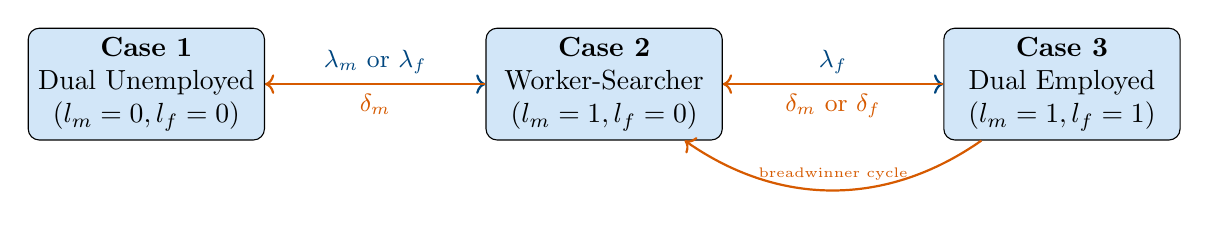
\begin{tikzpicture}[node distance=2.2cm, every node/.style={align=center}]
  \node[draw, fill=dutchlight, rounded corners, minimum width=3cm, minimum height=0.9cm]
    (UU) {\textbf{Case 1}\\Dual Unemployed\\$(l_m=0, l_f=0)$};
  \node[draw, fill=dutchlight, rounded corners, minimum width=3cm, minimum height=0.9cm, right=2.8cm of UU]
    (WS) {\textbf{Case 2}\\Worker-Searcher\\$(l_m=1, l_f=0)$};
  \node[draw, fill=dutchlight, rounded corners, minimum width=3cm, minimum height=0.9cm, right=2.8cm of WS]
    (EE) {\textbf{Case 3}\\Dual Employed\\$(l_m=1, l_f=1)$};

  \draw[->, thick, dutch] (UU) -- node[above, font=\small]{$\lambda_m$ or $\lambda_f$} (WS);
  \draw[->, thick, dutch] (WS) -- node[above, font=\small]{$\lambda_f$} (EE);
  \draw[->, thick, orange] (WS) -- node[below, font=\small]{$\delta_m$} (UU);
  \draw[->, thick, orange] (EE) -- node[below, font=\small]{$\delta_m$ or $\delta_f$} (WS);
  \draw[->, thick, orange, bend left=35] (EE) to node[above, font=\tiny]{breadwinner cycle} (WS);
\end{tikzpicture}
\end{center}
\vspace{0.5em}
%Each node has an associated value function over $(w_i, a^J, a_m, a_f, \theta)$. \\
All three cases are coupled by the \emph{joint} savings decision and the divorce threat.
\end{frame}

% ------------------------------------------------------------
\begin{frame}{Model: Case 1 — Dual Unemployed}
\small
Value function $U(b_m, b_f, a^J, a_m, a_f, \theta)$:
\begin{align*}
  \rho U(\cdot) = & \max_c \Bigg\{ u(c) + \lambda_m \int_{\underline{w}}^{\overline{w}} \max\{W_m(w,b_f,\cdot) - U(\cdot), 0\}\,dF_m(w) \\
    & + \lambda_f \int_{\underline{w}}^{\overline{w}} \max\{W_f(b_m,w,\cdot) - U(\cdot), 0\}\,dF_f(w) \\
    & + \mu_m \int [U(a, a_m{+}z, a_f, \theta) - U(\cdot)]\,dG_m(z) \\
    & + \mu_f \int [U(a, a_m, a_f{+}z, \theta) - U(\cdot)]\,dG_f(z) + \pi [V^D_m(\cdot) + V^D_f(\cdot) - U(\cdot)] \Bigg\}
\end{align*}

\vspace{0.2em}
\textbf{Reservation wages} $w^R_i$: defined implicitly by
$W_i(w^R_i, b_i, a^J, a_m, a_f, \theta) = U(b_m,b_f,a^J, a_m, a_f, \theta)$

\vspace{0.4em}
%\B{Insurance mechanism:} under $\theta = U$, divorce destroys $\tau_U$ of total wealth but distributes the rest equally — the \emph{same} regardless of who earned or inherited what. Under $\theta = L$, individual wealth shocks $z$ remain separate. \alert{This lowers the divorce continuation value for the lower-wealth spouse, reducing $U(\cdot)$ and hence the reservation wage.}
\end{frame}

% ------------------------------------------------------------
\begin{frame}{Model: Case 2 — Worker-Searcher}
\small
WLOG $l_m = 1,\, l_f = 0$. Value function $W_m(w_m,b_f, a^J, a_m, a_f, \theta)$:
\begin{align*}
\rho W_m(\cdot) = \max_{c,\, s_m} \Bigg\{&
u(c) - \kappa(s_m)
+ \delta_m [U(\cdot) - W_m(\cdot)]
+ s_m \gamma_m \int_{w_m}^{\overline{w}} [W_m(w,\cdot) - W_m(\cdot)]\,dF_m(w) \\
&+ \lambda_f \int \max\{E(w_m, w, \cdot) - W_m(\cdot),\; W_f(w,\cdot) - W_m(\cdot),\; 0\}\,dF_f(w) \\
&+ \mu_m \int [W_m(w_m, b_f, a^J, a_m{+}z, a_f, \theta) - W_m(\cdot)]\,dG_m(z) \\
&+ \mu_f \int [W_m(w_m, b_f, a^J, a_m, a_f{+}z, \theta) - W_m(\cdot)]\,dG_f(z)
+ \pi [V^D_m + V^D_f - W_m(\cdot)]
\Bigg\}
\end{align*}
\vspace{0.2em}
\textbf{Optimal on-the-job search:} FOC gives
$\kappa'(s_m^*(w_m)) = \gamma_m \int_{w_m}^{\overline{w}} [W_m(w,\cdot) - W_m(\cdot)]\,dF_m(w)$ \\
% review this!!!
\vspace{0.3em}
\B{Key:} under $\theta = L$, $\mu_f$ shock increases their separate wealth. It does not improve the employed spouse's divorce payoff. This asymmetry mutes the insurance benefit and lowers search intensity.
% Insurance mechanism operates through $U$ and $V^D$.
\end{frame}

% ------------------------------------------------------------
\begin{frame}{Model: Case 3 — Dual Employed}
\small
Value function $E(w_m, w_f, a^J, a_m, a_f, \theta)$:
\begin{align*}
\rho E(\cdot)=& \max_{c,s_m,s_f} \bigg\{u(c)-\kappa(s_m)-\kappa(s_f) \\
&+\delta_m\big[W_f(b_m,w_f,a^J,a_m,a_f,\theta)-E(\cdot)\big]\\&+\delta_f\big[W_m(w_m,b_f,a^J,a_m,a_f,\theta)-E(\cdot)\big]\\
&+s_m\gamma_m\int_{w_m}^{\overline{w}}\max\big\{E(w,w_f,a^J,a_m,a_f,\theta)-E(\cdot),W_m(w,b_f,a^J,a_m,a_f,\theta)-E(\cdot),0\big\}dF_m(w)\\
&+s_f\gamma_f\int_{w_f}^{\overline{w}}\max\big\{E(w_m,w,a^J,a_m,a_f,\theta)-E(\cdot),W_f(b_m,w,a^J,a_m,a_f,\theta)-E(\cdot),0\big\}dF_f(w)\\
&+\mu_m\int\big[E(w_m,w_f,a^J,a_m+z,a_f,\theta)-E(\cdot)\big]dG_m(z)\\&+\mu_f\int\big[E(w_m,w_f,a^J,a_m,a_f+z,\theta)-E(\cdot)\big]dG_f(z)\\
&+\pi\big[V_m^D(\cdot)+V_f^D(\cdot)-E(\cdot)]\bigg\}
\end{align*}
%\vspace{0.2em}
%\textbf{Optimal on-the-job search:} FOC gives
%$\kappa'(s_m^*(w_m)) = \gamma_m \int_{w_m}^{\overline{w}} [W_m(w,\cdot) - W_m(\cdot)]\,dF_m(w)$ \\
% review this!!!
%\vspace{0.3em}
%\B{Key:} under $\theta = L$, $\mu_f$ shock increases their separate wealth. It does not improve the employed spouse's divorce payoff. This asymmetry mutes the insurance benefit and lowers search intensity.
% Insurance mechanism operates through $U$ and $V^D$.
\end{frame}



\begin{frame}{Model: Divorce Value Functions}
\textbf{Divorce payoffs (key heterogeneity):} \\
\vspace{0.6em}
\begin{itemize}
\item If $\theta = U$ \\
$\to$ $a^D_i = \tfrac{1}{2}(1-\tau_U)(a^J + a_m + a_f)$\\[0.3em]
$\to$ Full pooling: wealth shocks shared equally regardless of recipient.\\
\vspace{1.6em}
\item If $\theta = L$ \\
$\to$ $a^D_i = \tfrac{1}{2}a^J + a_i$\\[0.3em]
$\to$ Partial pooling: only marital savings split; individual wealth and inheritances remain separate. \\
\end{itemize}
\vspace{1.6em}
$\tau_U > \tau_L = 0$: $U$ also entails higher dissolution costs
\end{frame}

% ------------------------------------------------------------
\begin{frame}{Model: Singles and Outside Option}

After divorce, each spouse becomes single with assets $a_i^D$. \\
\vspace{1.5em}

\textbf{Unemployed single:}
$\rho U^{\sin}_i(\cdot) = \max_{c_i}\left\{u(c_i) + \lambda_i \int \max\{E^{\sin}_i(w,a) - U_i(\cdot), 0\}\,dF_i(w)\right\}$

\vspace{1.5em}
\textbf{Employed single:}
$\rho E^{\sin}_i(\cdot) = u(c_i) - \kappa(s_i) + \delta_i[U^{\sin}_i(a) - E^{\sin}_i(\cdot)] + s_i\gamma_i \int [E^{\sin}_i(w', a) - E^{\sin}_i(\cdot)]\,dF_i(w')$ \\

\vspace{1.5em}
\textbf{Singles' reservation wage:} $U^{\sin}_i(a) = E^{\sin}_i(w^{R\sin}_i, a)$

%\vspace{0.5em}
%\begin{alertblock}{Why singles matter for the couple's problem}
%The divorce value functions $V^D_m, V^D_f$ embed the \emph{single} agent's value at the inherited asset level $a^D_i(\theta)$. The reform changes $a^D_i$ under $\theta = L$, which propagates back through the couple's value functions and alters search decisions \emph{throughout the marriage}.
%\end{alertblock}
\end{frame}


%\begin{frame}{Mechanism}

%Under universal property:

%\begin{itemize}
%    \item Divorce reallocates total wealth evenly
%    \item Higher effective insurance
%    \item Higher continuation value of unemployment
%    \item Higher reservation wages
%\end{itemize}

%Under limited property:

%\begin{itemize}
%    \item Wealth partially individualized
%    \item Divorce reduces expected wealth
%    \item Lower unemployment value
%    \item Lower reservation wages
%\end{itemize}

%\end{frame}
% ------------------------------------------------------------
%\begin{frame}{Model Summary: Mechanisms at a Glance}
%\begin{center}
%\begin{tikzpicture}[every node/.style={align=center, font=\small}]
%  \node[draw, fill=dutchlight, rounded corners, minimum width=3.2cm, minimum height=0.8cm] (reform)
%    at (0,0) {\textbf{Reform}: $\theta: U \to L$};

%  \node[draw, fill=white, rounded corners, minimum width=3.2cm, minimum height=0.8cm] (pool)
%    at (-4,-1.6) {Less asset pooling\\at divorce};
%  \node[draw, fill=white, rounded corners, minimum width=3.2cm, minimum height=0.8cm] (shock)
%    at (0,-1.6) {Wealth shocks\\stay individual};
%  \node[draw, fill=white, rounded corners, minimum width=3.2cm, minimum height=0.8cm] (cost)
%    at (4,-1.6) {Lower dissolution\\costs $\tau_L < \tau_U$};

%  \node[draw, fill=orange!15, rounded corners, minimum width=3.2cm, minimum height=0.8cm] (ins)
%    at (0,-3.2) {Lower effective\\marital insurance};

%  \node[draw, fill=dutch!15, rounded corners, minimum width=2.8cm, minimum height=0.8cm] (rw)
%    at (-3.5,-4.8) {Lower\\reservation wages};
%  \node[draw, fill=dutch!15, rounded corners, minimum width=2.8cm, minimum height=0.8cm] (si)
%    at (0,-4.8) {Less on-the-job\\search intensity};
%  \node[draw, fill=dutch!15, rounded corners, minimum width=2.8cm, minimum height=0.8cm] (sav)
%    at (3.5,-4.8) {More precautionary\\saving (individual)};

%  \foreach \s/\t in {reform/pool, reform/shock, reform/cost}
%    \draw[->, thick, dutch] (\s) -- (\t);
%  \foreach \s in {pool, shock, cost}
%    \draw[->, thick, dutch] (\s) -- (ins);
%  \foreach \t in {rw, si, sav}
%    \draw[->, thick, orange] (ins) -- (\t);
%\end{tikzpicture}
%\end{center}
%\end{frame}

\begin{frame}{Comparative Statics (Model Predictions)}

When insurance weakens:

\begin{itemize}
    \item $w_i^R \downarrow$
    \item Unemployment duration $\downarrow$
    \item On-the-job search intensity $\downarrow$
    \item Transitions into risky occupations $\downarrow$
\end{itemize}

\vspace{1.5em}
Strongest effects:
\begin{itemize}
    \item High premarital wealth asymmetry
    \item High divorce risk?
\end{itemize}

\end{frame}

% ------------------------------------------------------------
%\section{Identification \& Estimation}
% ------------------------------------------------------------
\begin{comment}
\begin{frame}{Identification Strategy}
\begin{columns}
\begin{column}{0.54\textwidth}
\textbf{Variation 1: Reform (DiD)}
\begin{itemize}
  \item Couples married \emph{before} 2018: $\theta = U$
  \item Couples married \emph{after} 2018: $\theta = L$
  \item Need to verify parallel pre-trends in job search outcomes
\end{itemize}
\vspace{0.5em}
\textbf{Variation 2: Wealth shocks (cross-sectional)}
\begin{itemize}
  \item Inheritances and gifts: $\mu_i \times G_i(z)$
  \item Under $U$: shock is shared; under $L$: stays individual
  \item Interact \emph{size} of wealth shock with regime indicator
  \item This variation traces the \emph{insurance} channel separately from a simple pre/post level comparison
\end{itemize}
\end{column}
\begin{column}{0.44\textwidth}
\begin{block}{Identification of model parameters}
\small
\begin{tabular}{ll}
\textbf{Parameter} & \textbf{Identified by}\\
\hline
$\delta_i, \lambda_i$ & Job transition rates\\
$F_i(w)$ & Accepted wage distribution\\
$\pi$ & Divorce hazard in data\\
$\tau_U$ & Asset division pre-2018\\
$\mu_i, G_i$ & Inheritance data\\
$\kappa_0, \kappa_1$ & Self-reported search effort + UE durations\\
$\rho$ & Asset decumulation during UE\\
\end{tabular}
\end{block}
\end{column}
\end{columns}
\end{frame}

% ------------------------------------------------------------
\begin{frame}{Estimation: SMM Approach}
\textbf{Simulated Method of Moments (SMM):}
\vspace{0.3em}

Minimize distance between model-simulated moments and data moments:
\[
\hat{\Theta} = \arg\min_\Theta \left[m_n - m(\Theta)\right]' W \left[m_n - m(\Theta)\right]
\]
\textbf{Proposed target moments:}
\begin{columns}
\begin{column}{0.50\textwidth}
\begin{itemize}
  \item Mean/variance of UE duration by regime
  \item Distribution of accepted wages (by regime)
  \item On-the-job search rates (job-to-job transitions)
  \item Self-reported reservation wages (DHS)
  \item Employment state transition rates
\end{itemize}
\end{column}
\begin{column}{0.50\textwidth}
\begin{itemize}
  \item Joint account share before/after reform
  \item Asset distribution at divorce
  \item Breadwinner cycle incidence
  \item Response of $\wR$ to inheritance shocks, by regime
  \item Divorce hazard by employment state
\end{itemize}
\end{column}
\end{columns}
\vspace{0.4em}
\small \alert{Key identifying restriction:} moments that respond to wealth shocks \emph{differently} pre- vs.\ post-2018 trace the insurance channel, conditional on the model.
\end{frame}
\end{comment}
% ------------------------------------------------------------
\section{Data}
% ------------------------------------------------------------

\begin{frame}{Data: DNB Household Survey (DHS)}
\textbf{Coverage:}
\begin{itemize}
  \item Dutch panel, $>$2,000 households/year, since 1993
  % research more on the data
  \item Work, pensions, housing, mortgages, income, health
  \begin{itemize}
    \item Self-reported \highlight{reservation wages}
    \item Unemployment duration
    \item Job-offer acceptance/rejection
    %\item Transitions to self-employment
  \end{itemize}
\end{itemize}
\vspace{0.8em}
\textbf{Wealth data:}
\begin{itemize}
  \item Assets, liabilities, account type: joint vs.\ individual
  \item Marital regime (default vs.\ settlement)
  \item Inheritance/gift receipt
\end{itemize}

\vspace{0.8em}
\small
\textbf{Limitation:}\\
After restricting to: (i) both spouses in labor force, (ii) classifying into dual-employed / worker-searcher / dual-unemployed $\Rightarrow$ \emph{sample shrinks substantially}.
\vspace{0.3em}

\end{frame}

% ------------------------------------------------------------
\begin{frame}{Data: CBS Microdata \& Linking Strategy}
\textbf{CBS (Statistics Netherlands) administrative microdata:}
\begin{itemize}
  \item Full-population panel: wages, employment spells, firm identifiers, tax records
  \item Regional housing price indices $\rightarrow$ premarital asset appreciation
  \item Sector-level unemployment rates $\rightarrow$ variation in $\lambda_i$ and $\delta_i$
\end{itemize}
\vspace{1.5em}
\textbf{Linking:}
\begin{itemize}
  \item DHS provides rich behavioral survey data (reservation wages, self-reported search)
  \item CBS provides statistical power and wealth shock measurement
\end{itemize}
\vspace{0.6em}
\small
\textbf{Current Idea}: Regional housing price indices can instrument for premarital wealth appreciation — a wealth shock that is (i) individual under $\theta = L$ but (ii) shared under $\theta = U$, and (iii) plausibly exogenous to individual job search decisions.
\end{frame}

% ------------------------------------------------------------
\begin{comment}
\begin{frame}{Preliminary Data Patterns}
\textcolor{red}{FIXXXX}  \\
\textbf{Marital status composition (Fig 1):}
\begin{itemize}
  \item Default (common property) $\approx 80\%$ of married couples across all years
  \item Share under marriage settlement $\approx 15$–$20\%$, stable over time
  \item No visible jump in settlements around 2018 $\Rightarrow$ supports exogeneity
\end{itemize}
\vspace{0.5em}
\textbf{Marriage type distribution (Fig 2):}
\begin{itemize}
  \item Married under default dominates
  \item Consistent with national statistics
  \item Key for DiD: treatment and control groups not selected into regimes based on reform
\end{itemize}

\end{frame}
\end{comment}

\begin{comment}
  \begin{enumerate}
  \item Pre-trends in reservation wages / UE durations pre-2018
  \item Distribution of joint account share over time
  \item Inheritance receipt rates by year and marital cohort
  \item Employment state distribution by regime
  \item Divorce hazard before and after reform
\end{enumerate}
\end{comment}

% ------------------------------------------------------------
\section{Additional Empirical Work}
% ------------------------------------------------------------

\begin{frame}{Suggested Additional Data Work (I)}
\textbf{1. Event-study / Staggered DiD around the 2018 Reform}
\begin{itemize}
  \item Use marriage cohort as the treatment timing variable
  \item Plot coefficients on year $\times$ post-2018 for: reservation wages, UE duration, job-to-job transitions
  %\item Tests parallel pre-trends %and maps the dynamic response of job search to the regime change
\end{itemize}
\vspace{1.5em}
\textbf{2. Inheritance / Gift Event Study}
\begin{itemize}
  \item Identify households receiving an inheritance shock 
  \item Plot job search outcomes in event time: $t-3, \ldots, t+3$ around receipt
  \item Compare responses under $\theta = U$ (pre-2018) vs.\ $\theta = L$ (post-2018)
  %\item Prediction: under $U$, inheritance raises $\wR$ (insured); under $L$, effect is smaller or asymmetric across spouses
\end{itemize}
\end{frame}

% ------------------------------------------------------------
\begin{frame}{Suggested Additional Data Work (II)}
%\textbf{3. Financial Pooling as a Continuous Treatment}
%\begin{itemize}
%  \item Construct $\text{pooling share} = a^J / (a^J + a_m + a_f)$ from DHS account data
%  \item Use as a continuous proxy for insurance intensity (within regime)
%  \item Instrument with regime indicator and premarital wealth $\Rightarrow$ 2SLS or structural first stage
%\end{itemize}
%\vspace{0.5em}
\textbf{3. Cohabiting Couples as a Control Group}
\begin{itemize}
  \item Cohabiting couples face no matrimonial property regime and have no automatic asset pooling
  %\item DHS has cohabitors: use as a ``pure separate'' benchmark to bound the insurance effect
  \item Test: do cohabitors' $\wR$ and search effort look like post-2018 married couples?
\end{itemize}
\vspace{1.5em}
\textbf{4. Housing Wealth Channel}
\begin{itemize}
  \item Homes are the dominant asset for Dutch couples
  \item Under $L$, premarital equity in the home is individual; under $U$ it is shared
  \item Use regional housing price appreciation as exogenous variation in premarital equity $\Rightarrow$ separate wealth shock from labor income shock
\end{itemize}
\end{frame}

% ------------------------------------------------------------
\begin{comment}
\begin{frame}{Suggested Additional Data Work (III)}
\textbf{6. Gender Asymmetry in Job Search Responses}
\begin{itemize}
  \item In Netherlands, gender wage gap implies women have lower premarital assets on average
  \item Under $U$: women benefit more from pooling with higher-earning husbands
  \item Prediction: reform should \emph{differentially} reduce $\wR$ and risk-taking for wives
  \item Test: heterogeneous treatment effects by relative wealth position of each spouse
\end{itemize}
\vspace{0.5em}
\textbf{7. Sector / Regional Unemployment Rate Interaction}
\begin{itemize}
  \item High-risk sectors (high $\delta_i$) should value insurance more
  \item Interact regime treatment with sector unemployment rate or local labor market tightness
  \item Prediction: reform depresses search behavior \emph{more} in high-risk sectors — directly tests the insurance channel
\end{itemize}
\vspace{0.5em}
\textbf{8. Precautionary Savings Response}
\begin{itemize}
  \item Model predicts: under $L$, individual account balances should rise (more precautionary saving)
  \item Test by comparing $\Delta a_i / \Delta a^J$ before vs.\ after reform among newly married cohorts
\end{itemize}
\end{frame}
\end{comment}
% ------------------------------------------------------------
\section{Counterfactuals \& Plan}
% ------------------------------------------------------------

\begin{frame}{Counterfactual Analysis (Post-Estimation)}
Once the model is estimated on pre- and post-2018 data:
\vspace{0.8em}
\begin{enumerate}
  %\item \textbf{Full reversion to universal CP:} simulate moving all post-2018 couples back to $\theta = U$\\
  %  $\Rightarrow$ recover the \emph{insurance value} of the reform in terms of reservation wages, UE durations, wage growth

  %\vspace{0.6em}
  \item \textbf{Shut down divorce risk ($\pi \to 0$):} isolate how much of the insurance mechanism runs through the \emph{divorce threat} vs.\ income pooling during marriage

  \vspace{0.6em}
  \item \textbf{Shut down wealth shocks ($\mu_i \to 0$):} what fraction of the regime effect operates through inheritance/gift risk?

  %\vspace{0.3em}
  %\item \textbf{Policy: means-tested divorce asset floor:} would a public insurance supplement offset the welfare loss of moving to $L$?

  %\vspace{0.3em}
  %\item \textbf{Aggregate labor market:} embed estimated behavioral responses in a search-and-matching framework — does the reform shift aggregate unemployment and wage inequality?
\end{enumerate}
\end{frame}

% ------------------------------------------------------------
\begin{comment}
\begin{frame}{Roadmap}
\begin{columns}
\begin{column}{0.50\textwidth}
\textbf{Step 1 (now):}
\begin{itemize}
  \item Finalize DHS descriptives; event-study pre-trends
  \item CBS linkage \& sample construction
\end{itemize}
\vspace{0.3em}
\textbf{Step 2:}
\begin{itemize}
  \item Solve model numerically (value function iteration)
  \item Characterize qualitative predictions
  \item Comparative statics on $\theta$, $\mu_i$, $\pi$
\end{itemize}
\vspace{0.3em}
\textbf{Step 3:}
\begin{itemize}
  \item SMM estimation — calibrate standard parameters from existing literature; estimate insurance/search parameters
  \item Informal and formal identification checks
\end{itemize}
\end{column}
\begin{column}{0.48\textwidth}
\textbf{Step 4:}
\begin{itemize}
  \item Counterfactual simulations
  \item Welfare analysis
\end{itemize}
\vspace{0.3em}
\textbf{Step 5:}
\begin{itemize}
  \item Robustness: alternative dissolution cost specifications, non-unitary bargaining extension, treatment of non-participation
\end{itemize}
\vspace{0.5em}
\begin{block}{Open questions for discussion}
\small
\begin{itemize}
  \item Unitary vs.\ Nash-bargaining model?
  \item How to handle labor force non-participation endogenously?
  \item Commingle rules — important to model explicitly?
\end{itemize}
\end{block}
\end{column}
\end{columns}
\end{frame}
\end{comment}
% ------------------------------------------------------------
\begin{frame}{Conclusion}
\textbf{What we do:}
\begin{itemize}
  \item Ask whether degree of marital insurance shapes job search behavior
  \item Exploit 2018 Dutch default property regime reform as quasi-experiment
  %\item Combine with inheritance shocks for cross-sectional identification
  \item Build a structural household search model 
\end{itemize}
\vspace{0.5em}
\textbf{Why it matters:}
\begin{itemize}
  \item Directly vary the institutional strength of marital insurance
  \item Provides causal evidence on the insurance mechanism at the core of household search theory
  %\item Policy implications: marriage law $\leftrightarrow$ labor market outcomes
\end{itemize}
\vspace{0.8em}
\textbf{Bottom line} \\
\small
Marriage law is labor market policy. Weakening asset pooling at divorce makes couples behave more like singles — even while still married. A structural model is needed to measure this.


\end{frame}

\bibliographystyle{plainnat}
\bibliography{bib}

\end{document}
